
\documentclass{beamer}
\usepackage[utf8]{inputenc}
\usepackage[spanish]{babel}
\usepackage{blindtext}
\usepackage{ragged2e}
\usepackage[numbers, sort, compress]{natbib}
\usepackage{graphicx}
\usepackage{multicol}
\usepackage{xcolor}
\usepackage{amsmath,amsfonts,amssymb}
    \allowdisplaybreaks[4]
\usepackage{subfig}
\usepackage{multirow}
\usepackage{array}
\usepackage{fancybox}
\usepackage{booktabs}

\definecolor{red_matrix}{rgb}{0.6, 0, 0}
\definecolor{green_matrix}{rgb}{0, 0.8, 0}
\definecolor{blue_matrix}{rgb}{0, 0.25, 1}

\usepackage{pifont}% http://ctan.org/pkg/pifont
	\newcommand{\cmark}{\color{green_matrix}\ding{51}}%
	\newcommand{\xmark}{\color{red}\ding{53}}%
\usepackage{tikz}
    \usetikzlibrary{arrows, matrix, calc,shapes.geometric,positioning}
\usepackage{setspace}
\usepackage{caption}
    \captionsetup[table]{font={normalsize,stretch=1.0}}
\usepackage{float}
\usepackage{adjustbox}
\usepackage{listings}

\setbeamertemplate{caption}[numbered]
\setbeamersize{description width=3.5cm}
\defbeamertemplate{description item}{align left}{\insertdescriptionitem\hfill}
\usetheme{Frankfurt}

%Information to be included in the title page:
\title{Detección de melanoma mediante\\ segmentación semántica}
\author{Mario Alberto Flores Hernández\\ 1719126 \\}
\institute{Asesora: Dra. Elisa Schaeffer \\Universidad Autónoma de Nuevo León \\Facultad de Ingeniería Mecánica y Eléctrica}
\date{2020}


\begin{document}

\frame{\titlepage}

\begin{frame}
    \frametitle{Índice}
    \vspace{-2cm}
    \begin{multicols}{2}
        \footnotesize{\tableofcontents}	
    \end{multicols}
\end{frame}

\section{Introducción}
\begin{frame}
    \frametitle{Introducción}
    La inteligencia artificial permite crear \textbf{modelos} que replican secuencias de transformaciones definidas por los datos entrantes.
    \begin{figure}
        \subfloat[Imagen Entrante\label{fig:a}]{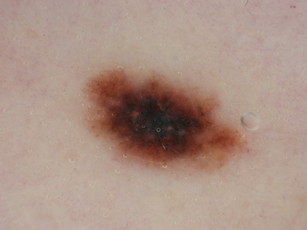
\includegraphics[height=4cm, width=4cm]{Figuras/input_1.png}} \qquad
        \subfloat[Salida Deseada\label{fig:b}]{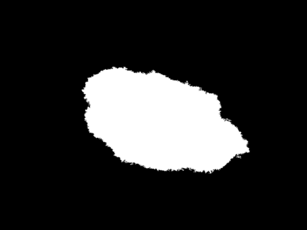
\includegraphics[height=4cm, width=4cm]{Figuras/mask_1.png}}
        \caption{Ejemplo de un modelo entrada-salida.}
    \end{figure}
\end{frame}

\subsection{Motivación}
\begin{frame}
    \frametitle{Motivación}
    Contribuir a la detección temprana del melanoma de piel para reducir la tasa de mortalidad.
\end{frame}

\subsection{Hipótesis}
\begin{frame}
    \frametitle{Hipótesis}
    Mediante la implementación de \textbf{redes neuronales convolucionales} e imágenes dermatológicas es posible entrenar modelos que repliquen la técnica de \textbf{segmentación semántica}, clasificando así las regiones dentro de la imagen. 
\end{frame}

\subsection{Objetivos}
\begin{frame}
    \frametitle{Objetivos}
    \begin{block}{Objetivos Generales}
        Implementar la tecnología de redes neuronales convolucionales con el fin de obtener un modelo cuya entrada sean imágenes dermatológicas y su salida sea un mapa probabilístico de las regiones dentro de ella.
        
    \end{block}
    \begin{block}{Objetivos Específicos}
        Determinar la secuencia de pre-procesamiento necesaria para adaptar imágenes de diferentes rangos de resolución a la resolución admitida por la arquitectura de la red neuronal convolucional y verificar la confiabilidad de la predicción mediante criterios de evaluación de mapas binarios y probabilísticos.
        
    \end{block}
\end{frame}

\section{Antecedentes}


\begin{frame}
\frametitle{Antecedentes}
    \begin{figure}
        \centering
        \subfloat[Blanco y Negro\label{fig:a}]{
            \begin{tikzpicture}
                \draw[step=5mm, black, line width=0.30mm] (-2,-2) grid (2,2);
                \node at (0,-2.5) {$\text{dim} = m \times n$};
            \end{tikzpicture}
        } \qquad
        \subfloat[Color\label{fig:b}]{
            \begin{tikzpicture}
                \draw[step=5mm, red_matrix, line width=0.30mm] (-2.5,-2.5) grid (1.5,1.5);
                \draw[step=5mm, green_matrix, line width=0.30mm] (-2,-2) grid (2,2);
                \draw[step=5mm, blue, line width=0.30mm] (-1.5,-1.5) grid (2.5,2.5);

                \node at (0, -3) {$\text{dim} = m \times n \times k$}; 
            \end{tikzpicture}
        }
        \caption{Características dimensionales de las imágenes.}
    \end{figure}
\end{frame}

\subsection{Función de Costo y Gradiente}
\begin{frame}
    \frametitle{Antecedentes}
    \begin{equation}\label{eq:dice_loss}
        \text{DL} = \frac{2|A \cap B |}{|A| + |B|}
    \end{equation}        
    
    \begin{equation}\label{eq:jacc}
        \text{IoU} = \frac{|A \cap B|}{| A \cup B |} = \frac{|A \cap B|}{|A| + |B| - |A \cap B|} \text{,}
      \end{equation}
      
    
\end{frame}

\section{Estado del Arte}

\subsection{Características}
\begin{frame}
    \frametitle{Estado del Arte}
    \setbeamertemplate{description item}[align left]
    \begin{description}
        \item[Clasificación]{Puede clasificar entre distintas categorías.}
        \item[Segmentación]{Puede segmentar las imágenes.}
        \item[Supervisado]{Requiere de datos de datos de entrenamiento.}
        \item[Pre-entrenamiento]{Puede inicializarse con pesos pre-entrenados como alternativa a la inicialización con pesos aleatorios.}
        \item[Evaluación]{Cuenta con una función de evaluación y un algoritmo de optimización.}
        \item[Salida]{Características de los datos obtenidos en la salida del modelo.}
    \end{description}
\end{frame}

\subsection{Literatura Revisada}
\begin{frame}
    \frametitle{Estado del Arte}

    \vspace{-0.5cm}

    \begin{table}[b!]
        \begin{center}
        \scalebox{0.65}{
            \begin{tabular}[t]{|l|l|l|l|l|l|l|l|}
                \hline
                \bf{Trabajo} & \bf{Modelo} & \bf{\rotatebox{90}{Clasificación}} & \bf{\rotatebox{90}{Segmentación}} & \bf{\rotatebox{90}{Supervisado}} & \bf{\rotatebox{90}{Pre-entrenamiento\phantom{m}}} & \bf{\rotatebox{90}{Evaluación}} & \bf{Salida}\\
                \hline
                \citet{DBLP:journals/corr/BadrinarayananK15} & \texttt{SegNet} & \cmark & \cmark & \cmark & \cmark & \cmark & mapa de etiquetas\\
                \citet{DBLP:journals/corr/RonnebergerFB15} & \texttt{U-net} & \cmark & \cmark & \cmark & \xmark & \cmark & mapa de etiquetas\\
                \citet{DBLP:journals/corr/ChenPK0Y16} & \texttt{DeepLab} & \cmark & \cmark & \cmark & \xmark & \cmark & mapa de etiquetas\\   
                \citet{DBLP:journals/corr/TeichmannWZCU16} & \texttt{MultiNet} & \cmark & \cmark & \cmark & \xmark & \cmark & mapa de etiquetas\\   
                \citet{KRONER2020261} & \texttt{VGG16} & \cmark & \cmark & \cmark & \cmark & \cmark & mapa de calor\\ 
                \citet{KADAMPUR2020100282} & \texttt{CNN} & \cmark & \xmark & \cmark & \xmark & \cmark & mapa de etiquetas\\    
                \citet{zhou2019emerging} & \texttt{ML / SVM} & \cmark & \xmark & \cmark & \xmark & \cmark & etiqueta\\    
                \citet{DBLP:journals/corr/LucCCV16} & \texttt{CNN/GAN} & \cmark & \cmark & \cmark & \cmark & \cmark & mapa de etiquetas\\         
                \citet{JAIN2015735} & \texttt{A.B.C.D} & \xmark & \cmark & \xmark & \xmark & \xmark & etiqueta\\
                \hline
                Propuesta de tesis & \texttt{FPN} & \cmark & \cmark & \cmark & \cmark & \cmark & mapa de etiquetas\\
                \hline   
            \end{tabular}
            }
        \end{center}
        \label{Tab:comp_1}
    \end{table}
\end{frame}

\section{Implementación}

\tikzstyle{decision} = [diamond, draw, fill=gray!20, 
    text width=5.5em, text badly centered, node distance=3cm, inner sep=0pt]
\tikzstyle{block} = [rectangle, draw, fill=gray!20, 
    text width=8em, text centered, rounded corners, minimum height=4em]
\tikzstyle{line} = [draw, -latex']
\tikzstyle{cloud} = [draw, ellipse,fill=red!20, node distance=3cm,
    minimum height=2em]

\subsection{Resolución Admitida}
\begin{frame}
    \frametitle{Implementación}
    \begin{figure}[b]
        \centering    
        \begin{tikzpicture}[node distance = 4cm, auto]
            % Nodos.
            \node [block] (init) {Cargado y Filtrado de Datos};
            \node [block, right of = init] (train) {Entrenamiento del Modelo};
            \node [block, right of = train] (pred) {Predicción de Máscaras};
            % Ejes.
            \path [line] (init) -- (train); 
            \path [line] (train) -- (pred); 
        \end{tikzpicture}
        \caption{Diagrama de flujo general de la herramienta propuesta.}
    \end{figure}

    \begin{block}{Resoluciones Admitidas}
        Las dimensiones de entrada admitidas por la red neuronal convolucional tienen que ser un múltiplo de 32, debído a que
        \begin{equation}
            \text{múltiplo} = 2^N
        \end{equation}
        donde $N$ es el número de capas del codificador de la red neuronal.
    \end{block}
\end{frame}

\subsection{Pre-procesado}
\begin{frame}
    \frametitle{Implementación}
    \begin{figure}[H]
        \centering
        \begin{adjustbox}{scale=0.8}
        \begin{tikzpicture}[node distance = 0.2cm and -1.5cm]
            \node [block] (input) {Imagen de Entrada \newline($m \times n$)};
            \node [block, below right=of input] (tr1) {Ajuste de tamaño ($512 \times 512$)};
            \node [block, below right= of tr1] (tr2) {Interpolación (\texttt{\small INTER$\_$AREA)}};
            \node [block, below right= of tr2] (tr3) {Transposición (2, 0, 1)};
            \node [block, below right= of tr3] (out) {Dato de Salida ($N \times (512 \times 512)$)};
            % Líneas
            \path [line] (input) -| (tr1);
            \path [line] (tr1) -| (tr2);
            \path [line] (tr2) -| (tr3);
            \path [line] (tr3) -| (out);
        \end{tikzpicture}
        \end{adjustbox}
        \caption{Línea de pre-procesamiento.}
        \label{fig: pipeline}
    \end{figure}
\end{frame}

\renewcommand{\lstlistingname}{Código}
\definecolor{codegreen}{rgb}{0,0.6,0}
\definecolor{codeblue}{rgb}{0.121, 0.203, 0.858}
\definecolor{codegray}{rgb}{0.5,0.5,0.5}
\definecolor{codepurple}{rgb}{0.58,0,0.82}
\definecolor{backcolour}{rgb}{0.95,0.95,0.92}

\lstdefinestyle{pystyle}{
    basicstyle= \scriptsize\ttfamily\linespread{1},
    backgroundcolor=\color{backcolour},   
    commentstyle=\color{codegreen},
    keywordstyle=\color{codeblue},
    numberstyle=\tiny\color{codegray},
    stringstyle=\color{codepurple},
    breakatwhitespace=false,         
    breaklines=true,                 
    captionpos=b,                    
    keepspaces=true,                 
    numbers=left,                    
    numbersep=5pt,                  
    showspaces=false,                
    showstringspaces=false,
    showtabs=false,                  
    tabsize=2
}

\lstset{style=pystyle}

\subsection{Entrenamiento}

\begin{frame}[fragile]
\frametitle{Implementación}
\begin{lstlisting}[language = Python, label = {code:train} ,caption= Búcle de entrenamiento. ]
# train_model.py
max_score = 0 
for i in range(0,40):
    print('\n Epoch: {}'.format(i))
    train_logs = train_epoch.run(train_loader)
    valid_logs = valid_epoch.run(valid_loader)
    if max_score < valid_logs['iou_score']:
        max_score = valid_logs['iou_score']
        torch.save(model,('Model/'+encoder+'.pth'))
        print('Highest Score Model Saved: {}'.format(max_score))
\end{lstlisting}
\end{frame}

\section{Experimentos}

\begin{frame}
    \frametitle{Experimentos}
    \setbeamertemplate{description item}[align left]
    \begin{description}
        \item[Filtro de umbral] Obtener el perfil de la \textbf{intensidad} de los pixeles antes y después del filtro.
        \item[Coeficiente de dados] Determinar el perfil del \textbf{error} durante la fase de entrenamiento.
        \item[Criterio de Jaccard] Determinar la \textbf{similitud} con mayor penalización del error en la fase de validación.   
    \end{description}
\end{frame}


\subsection{Filtrado de Umbral}
\begin{frame}
    \frametitle{Experimentos}
    \begin{figure}
        \centering
        \subfloat[Imagen Entrante\label{fig:a}]{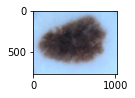
\includegraphics[scale=0.5]{../Plots/THR/sample_0.png}} \qquad
        \subfloat[Imagen Filtrada\label{fig:b}]{\hspace{0.35cm}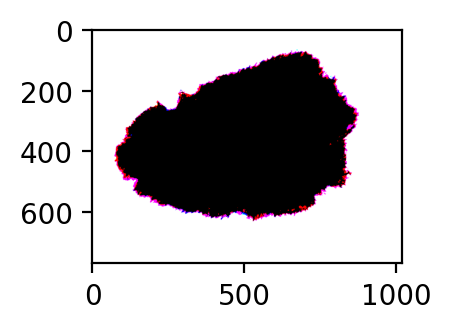
\includegraphics[scale=0.5]{../Plots/THR/filtered_0.png}} \\
        \subfloat[Histograma Original\label{fig:c}]{\hspace{0.7cm}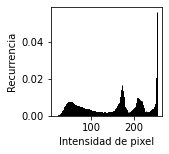
\includegraphics[scale=0.5]{../Plots/THR/threshold_input_0.png}\hspace{0.3cm}} \qquad
        \subfloat[Histograma Resultante\label{fig:c}]{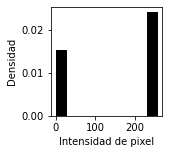
\includegraphics[scale=0.5]{../Plots/THR/threshold_output_0.png}\hspace{1cm}}
        \caption{Filtrado de umbral antes y después.}
    \end{figure}
\end{frame}

\subsection{Coeficiente de Dados}
\begin{frame}
    \frametitle{Experimentos}
    \begin{figure}
        \centering
        \subfloat[Época 1\label{fig:a}]{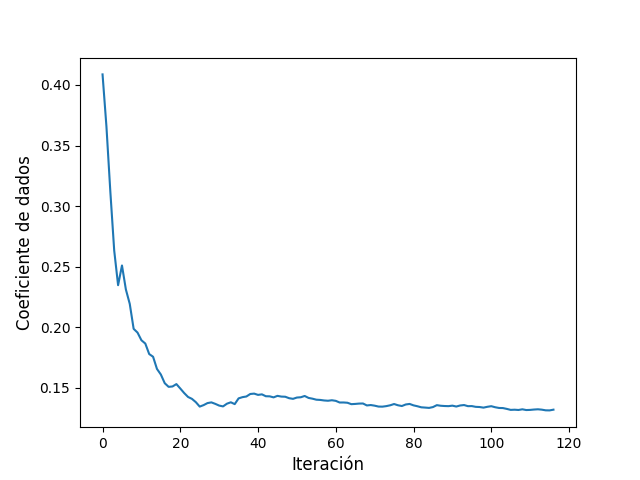
\includegraphics[height=2.5cm, width=2.5cm]{../Plots/dl_epoch_0.png}} \qquad
        \subfloat[Época 2\label{fig:b}]{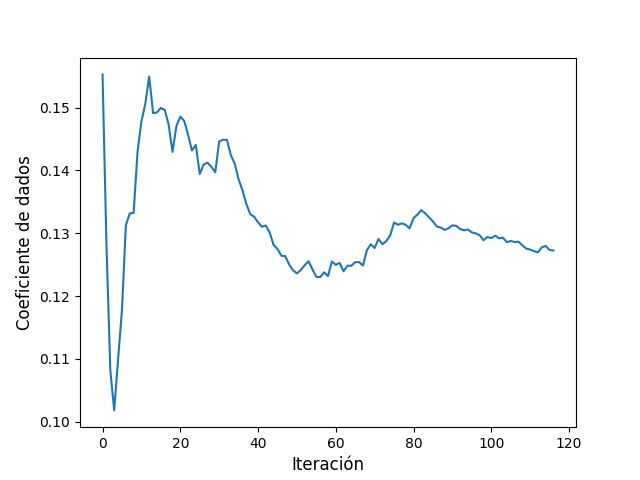
\includegraphics[height=2.5cm, width=2.5cm]{../Plots/dl_epoch_1.png}} \qquad
        \subfloat[Época 3\label{fig:c}]{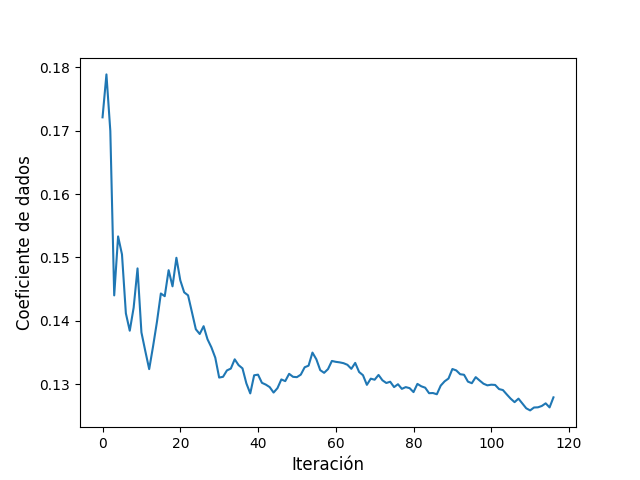
\includegraphics[height=2.5cm, width=2.5cm]{../Plots/dl_epoch_2.png}} \\
        \subfloat[Época 4\label{fig:a}]{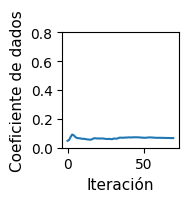
\includegraphics[height=2.5cm, width=2.5cm]{../Plots/dl_epoch_3.png}} \qquad
        \subfloat[Época 5\label{fig:b}]{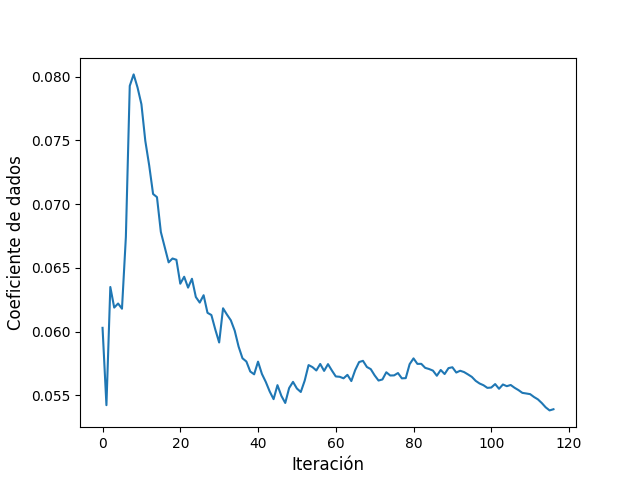
\includegraphics[height=2.5cm, width=2.5cm]{../Plots/dl_epoch_4.png}} \qquad
        \subfloat[Época 6\label{fig:c}]{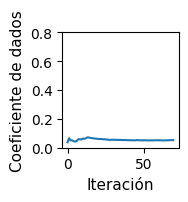
\includegraphics[height=2.5cm, width=2.5cm]{../Plots/dl_epoch_5.png}} \\
        \caption{Error según el coeficiente de dados.}
    \end{figure}
\end{frame}

\subsection{Criterio de Jaccard}
\begin{frame}
    \frametitle{Experimentos}
    \begin{figure}
        \centering
        \subfloat[Época 1\label{fig:a}]{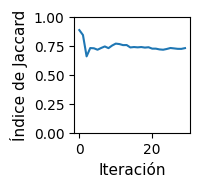
\includegraphics[height=2.5cm, width=2.5cm]{../Plots/score_epoch_0.png}} \qquad
        \subfloat[Época 2\label{fig:b}]{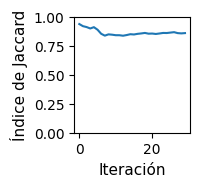
\includegraphics[height=2.5cm, width=2.5cm]{../Plots/score_epoch_1.png}} \qquad
        \subfloat[Época 3\label{fig:c}]{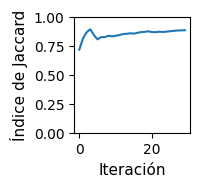
\includegraphics[height=2.5cm, width=2.5cm]{../Plots/score_epoch_2.png}} \\
        \subfloat[Época 4\label{fig:a}]{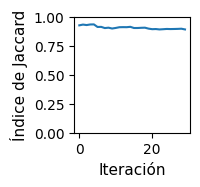
\includegraphics[height=2.5cm, width=2.5cm]{../Plots/score_epoch_3.png}} \qquad
        \subfloat[Época 5\label{fig:b}]{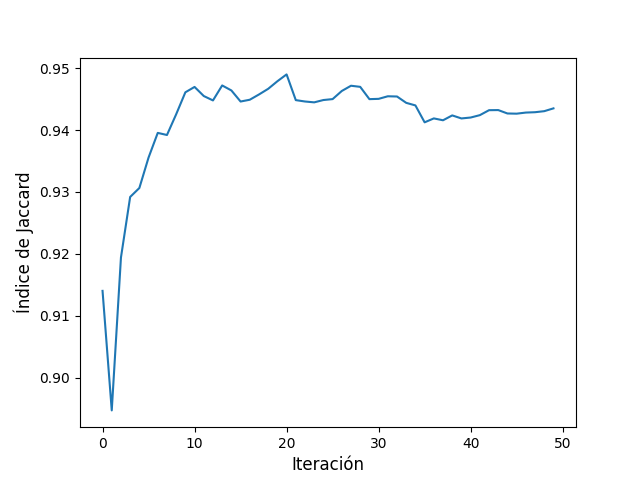
\includegraphics[height=2.5cm, width=2.5cm]{../Plots/score_epoch_4.png}} \qquad
        \subfloat[Época 5\label{fig:c}]{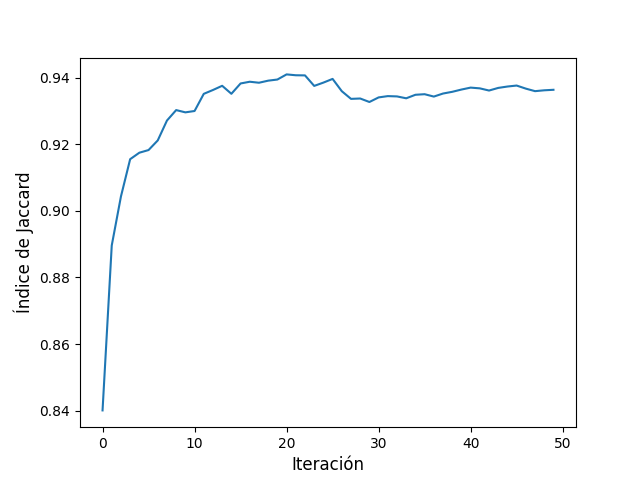
\includegraphics[height=2.5cm, width=2.5cm]{../Plots/score_epoch_5.png}} \\
        \caption{Similitud según el criterio de Jaccard.}
    \end{figure}
\end{frame}

\begin{frame}
    \frametitle{Resultados}

    \begin{table}
        \centering
        \caption{Resultados de criterios por época.}
        \begin{tabular}{c c c}
          \toprule
          \textbf{Epoch} & \textbf{DL} & \textbf{IoU} \\
          \midrule
          1 & 0.2968 & 0.5616 \\
          2 & 0.2972 & 0.5546 \\
          3 & 0.2690 & 0.5879 \\
          4 & 0.2960 & 0.6389 \\
          5 & 0.2371 & 0.8415 \\
          6 & 0.0929 & 0.8626 \\
          7 & 0.0792 & 0.8626 \\
          8 & 0.0692 & 0.8798 \\
          9 & 0.0556 & 0.9017 \\
          10 & 0.0542 & 0.9039 \\
          \bottomrule
          
        \end{tabular}
        \label{table:summary}
      \end{table}
\end{frame}

\begin{frame}
    \frametitle{Resultados}
    \begin{figure}
        \centering
        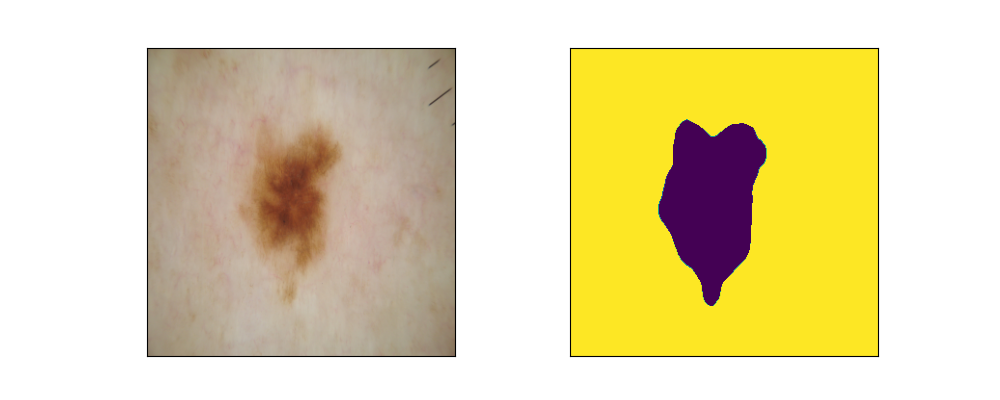
\includegraphics[scale=0.4]{Figure_1.png}
        \caption{Imagen entrante y máscara generada por el modelo.}
    \end{figure}
\end{frame}

\section{Conclusión}
\subsection{Discusión}
\begin{frame}
    \frametitle{Conclusión}
    La implementación de la red neuronal convolucional y el entrenamiento del modelo cumplieron satisfactoriamente con la hipótesis establecida al estimar con un 96\% de precisión las máscaras en el conjunto de datos de pruebas.
\end{frame}


\subsection{Trabajo a Futuro}
\begin{frame}
    \frametitle{Trabajo a Futuro}
    Trabajar con redes neuronales de segmentación semántica instanciada para la detección de múltiples instancias de los objetos dentro de la misma categoría. 
\end{frame}

\subsection{Agradecimientos}
\begin{frame}
    \frametitle{Agradecimientos}
    Agradecimientos a la Dra. Satu Elisa Schaeffer por su asesoría, al comité de revisores formado por la Dra. Sara Elena Garza Villarreal y el Dr. Romeo Sánchez Nigenda por el tiempo y la dedicación que me otorgaron mediante sus observaciones.
\end{frame}

\begin{frame}[allowframebreaks]
    \footnotesize
    \nocite{adam_opt}
    \frametitle{Referencias}
    \bibliographystyle{mighelnat}
    \bibliography{MiBiblio}
    
    
\end{frame}

\end{document}